\documentclass[11pt,a4paper]{article}

%% ---------------------------------------------------------------- packages
\usepackage[utf8]{inputenc}
\usepackage[T1]{fontenc}
\usepackage[english]{babel}
\usepackage[a4paper,margin=2.5cm]{geometry}
\usepackage{amsmath,amssymb}
\usepackage{siunitx}
\usepackage{booktabs}
\usepackage{graphicx}
\usepackage{caption}
\usepackage{subcaption}
\usepackage{enumitem}
\usepackage{xcolor}
\usepackage[hidelinks]{hyperref}

\sisetup{detect-all, per-mode=symbol}
\captionsetup{font=small, labelfont=bf}
\setlength{\parindent}{0pt}
\setlength{\parskip}{0.6em}
\numberwithin{equation}{section}

%% ---------------------------------------------------------------- shortcuts
\newcommand{\Cd}{C_d}
\newcommand{\Red}{\mathrm{Re}_d}
\newcommand{\ey}{\mathbf{e}_y}
\newcommand{\ex}{\mathbf{e}_x}
\newcommand{\Fth}{F_{\mathrm{th}}}

\begin{document}

%% ================================================================ COVER
\begin{titlepage}
\centering
\vspace*{1.5cm}
\IfFileExists{logo_uc3m.png}{\includegraphics[width=4.2cm]{logo_uc3m.png}\\[1.2cm]}{\vspace*{1.5cm}}
{\Huge\scshape Universidad Carlos III de Madrid\par}
\vspace{0.4cm}
{\large Aerospace Engineering\par}
\vspace{1.2cm}
{\Large UC3M\par}
\vspace{0.8cm}
\rule{\linewidth}{1.2pt}\\[0.3cm]
{\LARGE\bfseries Jet Impact on Surfaces\par}
\vspace{0.3cm}
\rule{\linewidth}{1.2pt}\\[0.8cm]
{\large Fluid Mechanics --- Laboratory Session Report\par}
\vspace{1.2cm}
\begin{flushleft}
\hspace{1.2cm}\textit{Authors:}\\
\hspace{1.2cm}Marcos Guijarro Ruano\\
\hspace{1.2cm}Alejandro Ranz Remart\'inez\\
\hspace{1.2cm}Aimar \'Alvarez Iglesias\\
\hspace{1.2cm}H\'ector Gonz\'alez Rodr\'iguez\\
\hspace{1.2cm}Ismael Mart\'in D\'iez
\end{flushleft}
\vspace{1cm}
{\large\textbf{Report date:} September 30, 2026}
\vfill
\end{titlepage}



\tableofcontents
\newpage

%% ================================================================ 1 INTRODUCTION
\section{Introduction}

When a liquid jet is turned by a solid surface, the change in its linear momentum must be supplied by a force on that surface. This momentum transfer is one of the ways in which fluid streams produce loads, and it can be quantified without solving for the detailed flow in the impact region: only the fluxes of momentum across the boundaries of a suitably chosen control volume are needed.

The specific objectives of this session are:
\begin{enumerate}[leftmargin=1.5em, itemsep=0.2em]
  \item to derive, from the continuity and momentum equations applied to a control volume, the force exerted by a jet on a flat plate, a $30^\circ$ oblique surface and a hemispherical surface;
  \item to measure that force experimentally by balancing it with calibrated masses for several flow rates;
  \item to compare $F(Q)$ with the theoretical predictions and to compute the drag coefficient $\Cd$ of each obstacle as a function of the Reynolds number $\Red$;
  \item to quantify the measurement uncertainty and to diagnose the physical origin of the discrepancies.
\end{enumerate}

%% ================================================================ 2 THEORY
\section{Theoretical Derivation of the Jet Impact Force}
\subsection{Control Volume Formulation and Bernoulli Equation}
Consider the control volume bounded by the closed surface $\Sigma_c = \Sigma_i + \Sigma_o + \Sigma_l + \Sigma_w$, where:
\begin{itemize}
    \item $\Sigma_i$: the inlet jet surface arriving to the plate (area $A_i$).
    \item $\Sigma_o$: the outlet jet surface exiting the water sheet (area $A_o$).
    \item $\Sigma_l$: the lateral surface of the jet exposed to atmospheric pressure ($p = p_a$).
    \item $\Sigma_w$: the contact surface on the obstacle.
\end{itemize}

 Applying Bernoulli's equation to the streamline from the nozzle exit to the sheet exit and neglecting the effect of gravity:
\begin{equation}
    \frac{p_a}{\rho} + \frac{v_i^2}{2} = \frac{p_a}{\rho} + \frac{v_o^2}{2} \implies v_i = v_o = v = \frac{Q}{A}
\end{equation}

\subsection{Conservation of Mass (Mass Continuity Equation)}
For steady, incompressible flow through the control surface $\Sigma_c$:
\begin{equation}
    \iint_{\Sigma_c} \rho (\vec{v} \cdot \vec{n}) \, d\sigma = 0
\end{equation}
Splitting across the boundary surfaces:
\begin{equation}
    \iint_{\Sigma_i} \rho (\vec{v} \cdot \vec{n}) \, d\sigma + \iint_{\Sigma_o} \rho (\vec{v} \cdot \vec{n}) \, d\sigma + \iint_{\Sigma_l} \rho (\vec{v} \cdot \vec{n}) \, d\sigma + \iint_{\Sigma_w} \rho (\vec{v} \cdot \vec{n}) \, d\sigma = 0
\end{equation}
Since $\vec{v} \cdot \vec{n} = 0$ in the stream surfaces $\Sigma_l$ and $\Sigma_w$, with $\vec{v}_i = v_i \vec{e}_y$, $\vec{n}_i = -\vec{e}_y$, and $\vec{v}_o \cdot \vec{n}_o = v_o$:
\begin{equation}
    -\rho v_i A_i + \rho v_o A_o = 0 \implies \rho v_i A_i = \rho v_o A_o
\end{equation}
Since $v_i = v_o = v$, it follows that:
\begin{equation}
    A_i = A_o = A
\end{equation}

\subsection{Conservation of Linear Momentum}
The conservation of linear momentum equation applied to the control volume $\Sigma_c$ neglecting the effects of the viscous and gravity forces is:
\begin{equation}
    \iint_{\Sigma_c} \rho \vec{v} (\vec{v} \cdot \vec{n}) \, d\sigma = -\iint_{\Sigma_c} (p - p_a) \vec{n} \, d\sigma
\end{equation}
Along the different surfaces:
\begin{equation}
    -\iint_{\Sigma_c} (p - p_a) \vec{n} \, d\sigma = -\underbrace{\iint_{\Sigma_i}(p_a - p_a)\vec{n}\,d\sigma}_{0} - \underbrace{\iint_{\Sigma_o}(p_a - p_a)\vec{n}\,d\sigma}_{0} - \underbrace{\iint_{\Sigma_l}(p_a - p_a)\vec{n}\,d\sigma}_{0} - \iint_{\Sigma_w}(p - p_a)\vec{n}\,d\sigma
\end{equation}
The force exerted by the jet on the obstacle accounts for the atmospheric pressure $p_a$ acting on the upper face of the obstacle:
\begin{equation}
    \vec{F} = \iint_{\Sigma_w} (p - p_a) \vec{n} \, d\sigma \implies -\iint_{\Sigma_c} (p - p_a) \vec{n} \, d\sigma = -\vec{F}
\end{equation}
Therefore, the momentum equation reduces to:
\begin{equation}
    \iint_{\Sigma_i} \rho \vec{v} (\vec{v} \cdot \vec{n}) \, d\sigma + \iint_{\Sigma_o} \rho \vec{v} (\vec{v} \cdot \vec{n}) \, d\sigma = -\vec{F}
\end{equation}

\subsection{Evaluation of the Force on the Three Geometries}

\paragraph{Flat Surface ($\beta = 90^\circ$)}
At the inlet $\vec{v}_i = v_i \vec{e}_y$ with $\vec{n}_i = -\vec{e}_y$. At the outlet, the fluid leaves purely horizontally along the plate: $\vec{v}_o = v_o \vec{e}_x$ with $\vec{v}_o \cdot \vec{n}_o = v_o$:
\begin{equation}
    \int_{\Sigma_i} \rho (v_i \vec{e}_y)(-v_i) \, d\sigma + \rho v_o^2 A_o \vec{e}_x = -\vec{F}
\end{equation}
\begin{equation}
    -\rho v_i^2 A_i \vec{e}_y + \rho v_o^2 A_o \vec{e}_x = -\vec{F} \implies \vec{F} = \rho v_i^2 A_i \vec{e}_y - \rho v_o^2 A_o \vec{e}_x
\end{equation}
Projecting along the vertical direction $\vec{e}_y$:
\begin{equation}
    F_y = \rho v_i^2 A_i = \rho v^2 A = \rho \left(\frac{Q}{A}\right)^2 A = \rho \frac{Q^2}{A}
    \label{eq:flat_force}
\end{equation}

\paragraph{Oblique Surface ($\alpha = 30^\circ$)}
The water sheet leaves inclined at an angle of $30^\circ$ below the horizontal:
\begin{equation}
    \vec{v}_o = v_o \cos\left(\frac{\pi}{6}\right) \vec{e}_x - v_o \sin\left(\frac{\pi}{6}\right) \vec{e}_y, \quad \text{with } \vec{v}_o \cdot \vec{n}_o = v_o
\end{equation}
Substituting into the momentum balance:
\begin{equation}
    -\rho v_i^2 A_i \vec{e}_y + \int_{\Sigma_o} \rho \left( v_o \cos\left(\frac{\pi}{6}\right)\vec{e}_x - v_o \sin\left(\frac{\pi}{6}\right)\vec{e}_y \right) v_o \, d\sigma = -\vec{F}
\end{equation}
\begin{equation}
    \vec{F} = \rho v_i^2 A_i \vec{e}_y + \rho v_o^2 \cos\left(\frac{\pi}{6}\right) A_o \vec{e}_x + \rho v_o^2 \sin\left(\frac{\pi}{6}\right) A_o \vec{e}_y
\end{equation}
Since $\sin(\pi/6) = \frac{1}{2}$ and $v_i = v_o = v$, $A_i = A_o = A$, the vertical force $F_y$ is:
\begin{equation}
    F_y = \left(1 + \sin\left(\frac{\pi}{6}\right)\right) \rho v^2 A = \left(1 + \frac{1}{2}\right) \rho v^2 A = \frac{3}{2} \rho \frac{Q^2}{A}
\end{equation}

\paragraph{Hemispherical Surface ($\beta = 180^\circ$)}
The water sheet exits directed completely downwards: $\vec{v}_o = -v_o \vec{e}_y$ with $\vec{n}_o = -\vec{e}_y$, so $\vec{v}_o \cdot \vec{n}_o = (-v_o \vec{e}_y) \cdot (-\vec{e}_y) = v_o$:
\begin{equation}
    \int_{\Sigma_i} \rho (v_i \vec{e}_y)(-v_i) \, d\sigma + \int_{\Sigma_o} \rho (-v_o \vec{e}_y)(v_o) \, d\sigma = -\vec{F}
\end{equation}
\begin{equation}
    -\rho v_i^2 A_i \vec{e}_y - \rho v_o^2 A_o \vec{e}_y = -\vec{F}
\end{equation}
\begin{equation}
    \vec{F} = 2\rho v^2 A \vec{e}_y \implies F_y = 2\rho v^2 A = 2\rho \frac{Q^2}{A}
\end{equation}
\subsection{Drag Coefficient ($C_{\mathrm{d}}$)}

If we define the drag coefficient as the dimensionless number:
\begin{equation}
    C_{\mathrm{d}} = \frac{F}{\frac{1}{2}\rho v^{2} A}
    \label{eq:cd_definition}
\end{equation}
substituting the vertical force expressions derived for each geometry:

\begin{itemize}
    \item \textbf{Flat surface} ($F = \rho v^{2} A = \rho \frac{Q^2}{A}$):
    \begin{equation}
        C_{\mathrm{d}} = \frac{\rho v^{2} A}{\frac{1}{2}\rho v^{2} A} = 2
    \end{equation}

    \item \textbf{Oblique surface} ($F = \frac{3}{2}\rho v^{2} A = 1.5 \rho \frac{Q^2}{A}$):
    \begin{equation}
        C_{\mathrm{d}} = \frac{\frac{3}{2}\rho v^{2} A}{\frac{1}{2}\rho v^{2} A} = 3
    \end{equation}

    \item \textbf{Hemispherical surface} ($F = 2\rho v^{2} A = 2\rho \frac{Q^2}{A}$):
    \begin{equation}
        C_{\mathrm{d}} = \frac{2\rho v^{2} A}{\frac{1}{2}\rho v^{2} A} = 4
    \end{equation}
\end{itemize}
Thus, the theoretical drag coefficients take the constant values $C_{\mathrm{d}} = 2$ for the flat surface, $C_{\mathrm{d}} = 3$ for the oblique surface, and $C_{\mathrm{d}} = 4$ for the hemispherical surface.
%% ================================================================ 3 APPARATUS
\section{Experimental Apparatus and Test Procedure}

\subsection{Apparatus}

To quantify the momentum transfer, the experiment was performed on an Edibon hydraulic bench providing a continuous water supply through an internal closed circuit. A vertical nozzle with an inner diameter of $d = \SI{8}{\milli\meter}$ directs the jet toward the obstacle inside a test cylinder. Three interchangeable geometries were tested: a flat plate ($90^\circ$ radial deflection), a $30^\circ$ conical one, and a hemispherical cup ($180^\circ$ flow reversal). The experimental flow rate was monitored through the rotameter panel in $\si{L/h}$, with the spent fluid draining continuously from the chamber base.

The reaction force is measured using a counterbalanced lever system. The rod supporting the test body is coupled to a horizontal balance disk, opposite a loading platform. Before each run, the disk was leveled, and the gauge was aligned with an extra reference mark. Calibrated weights were then added to the pan in $\SI{50}{\gram}$ steps. By adjusting the supply valve, the flow rate was regulated until the beam returned to its baseline alignment mark, ensuring that the hydrodynamic impact force directly equilibrated the countermass weight ($F = mg$).
\begin{figure}[htbp]
\centering
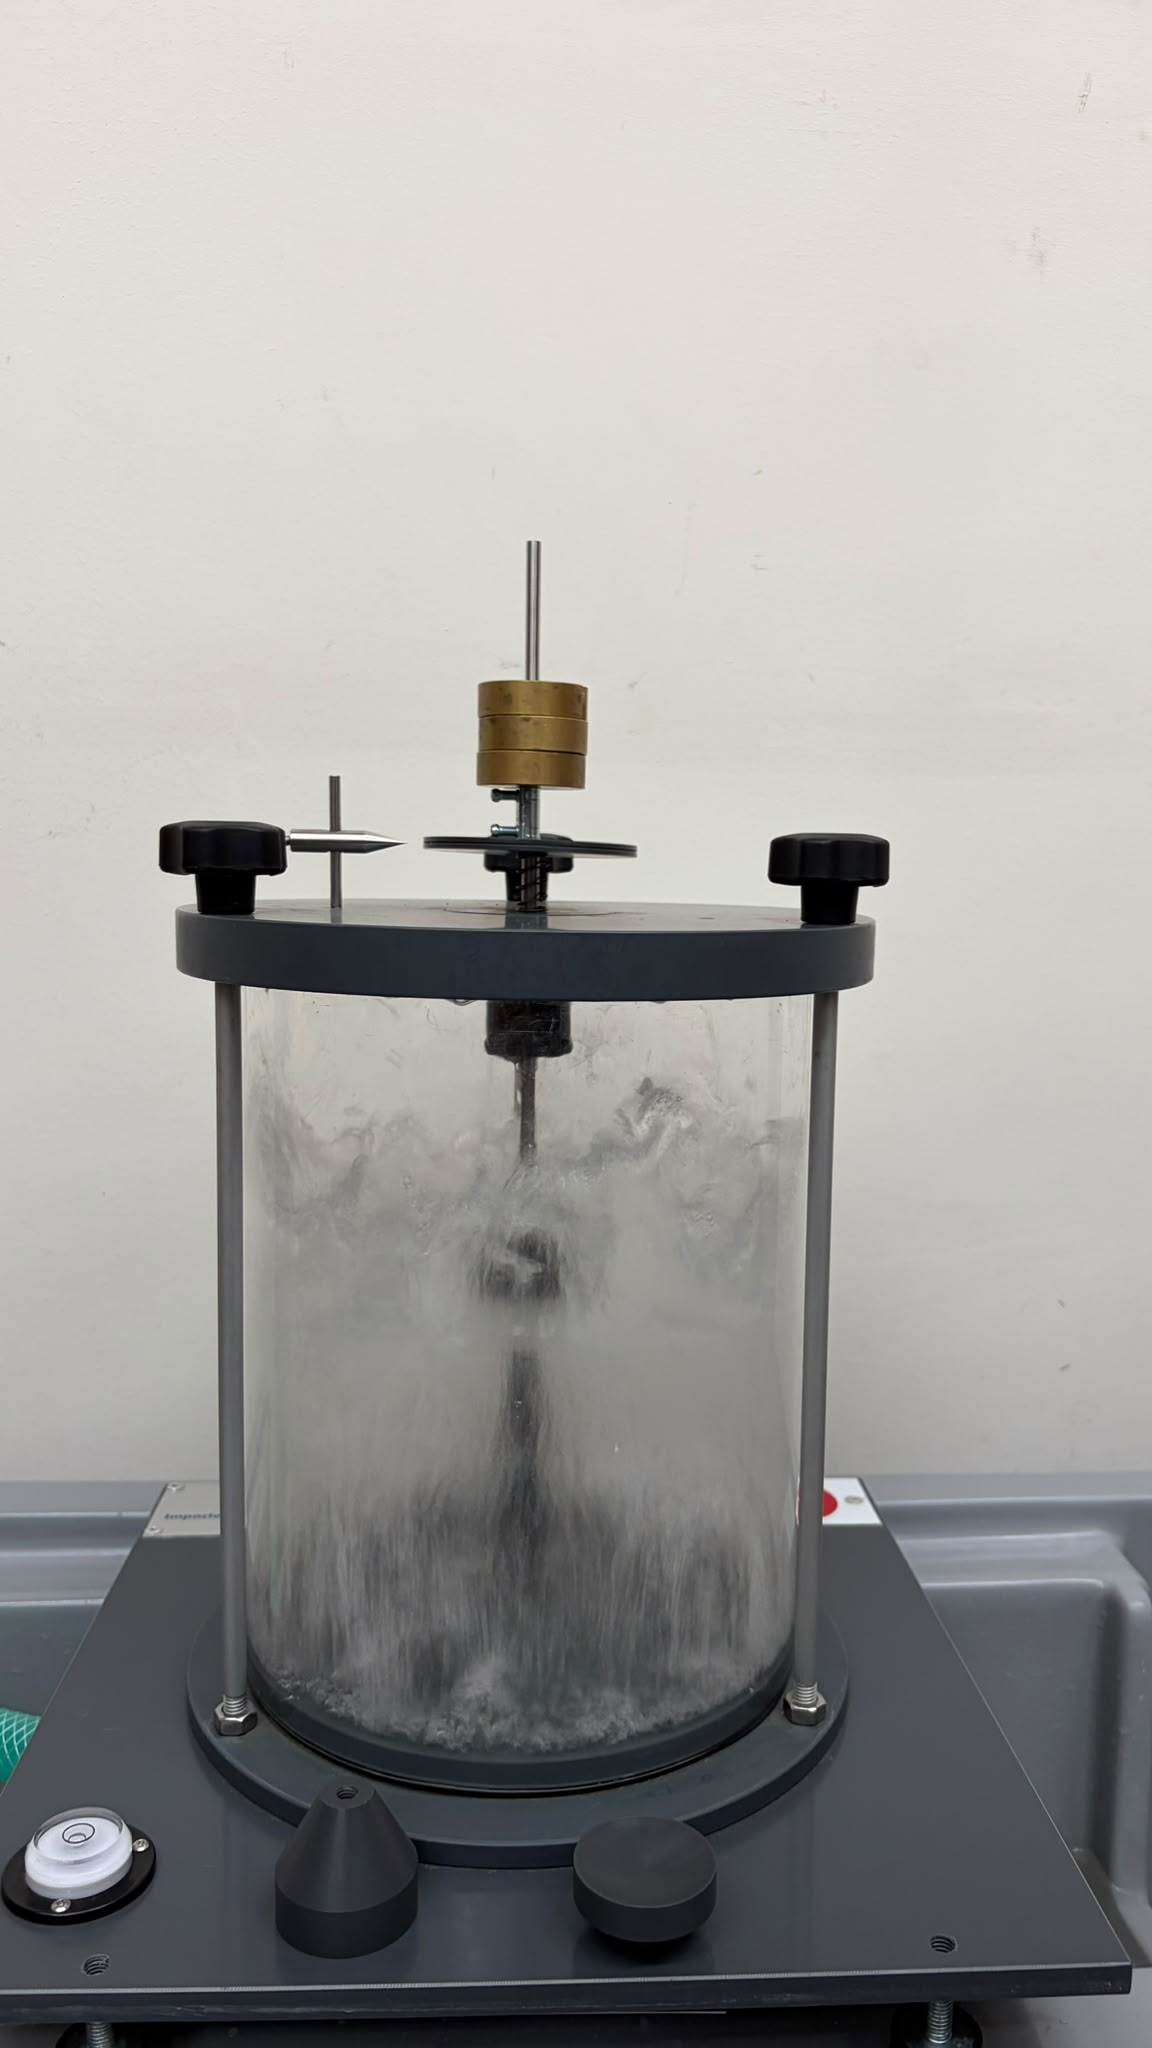
\includegraphics[width=0.20\linewidth]{Aparatus.jpeg}
\caption{Jet impact experimental setup during flow measurement, balanced with calibrated weights.}
\label{fig:cd}
\end{figure}

\begin{figure}[htbp]
    \centering
    \begin{subfigure}[t]{0.35\textwidth}
        \centering
        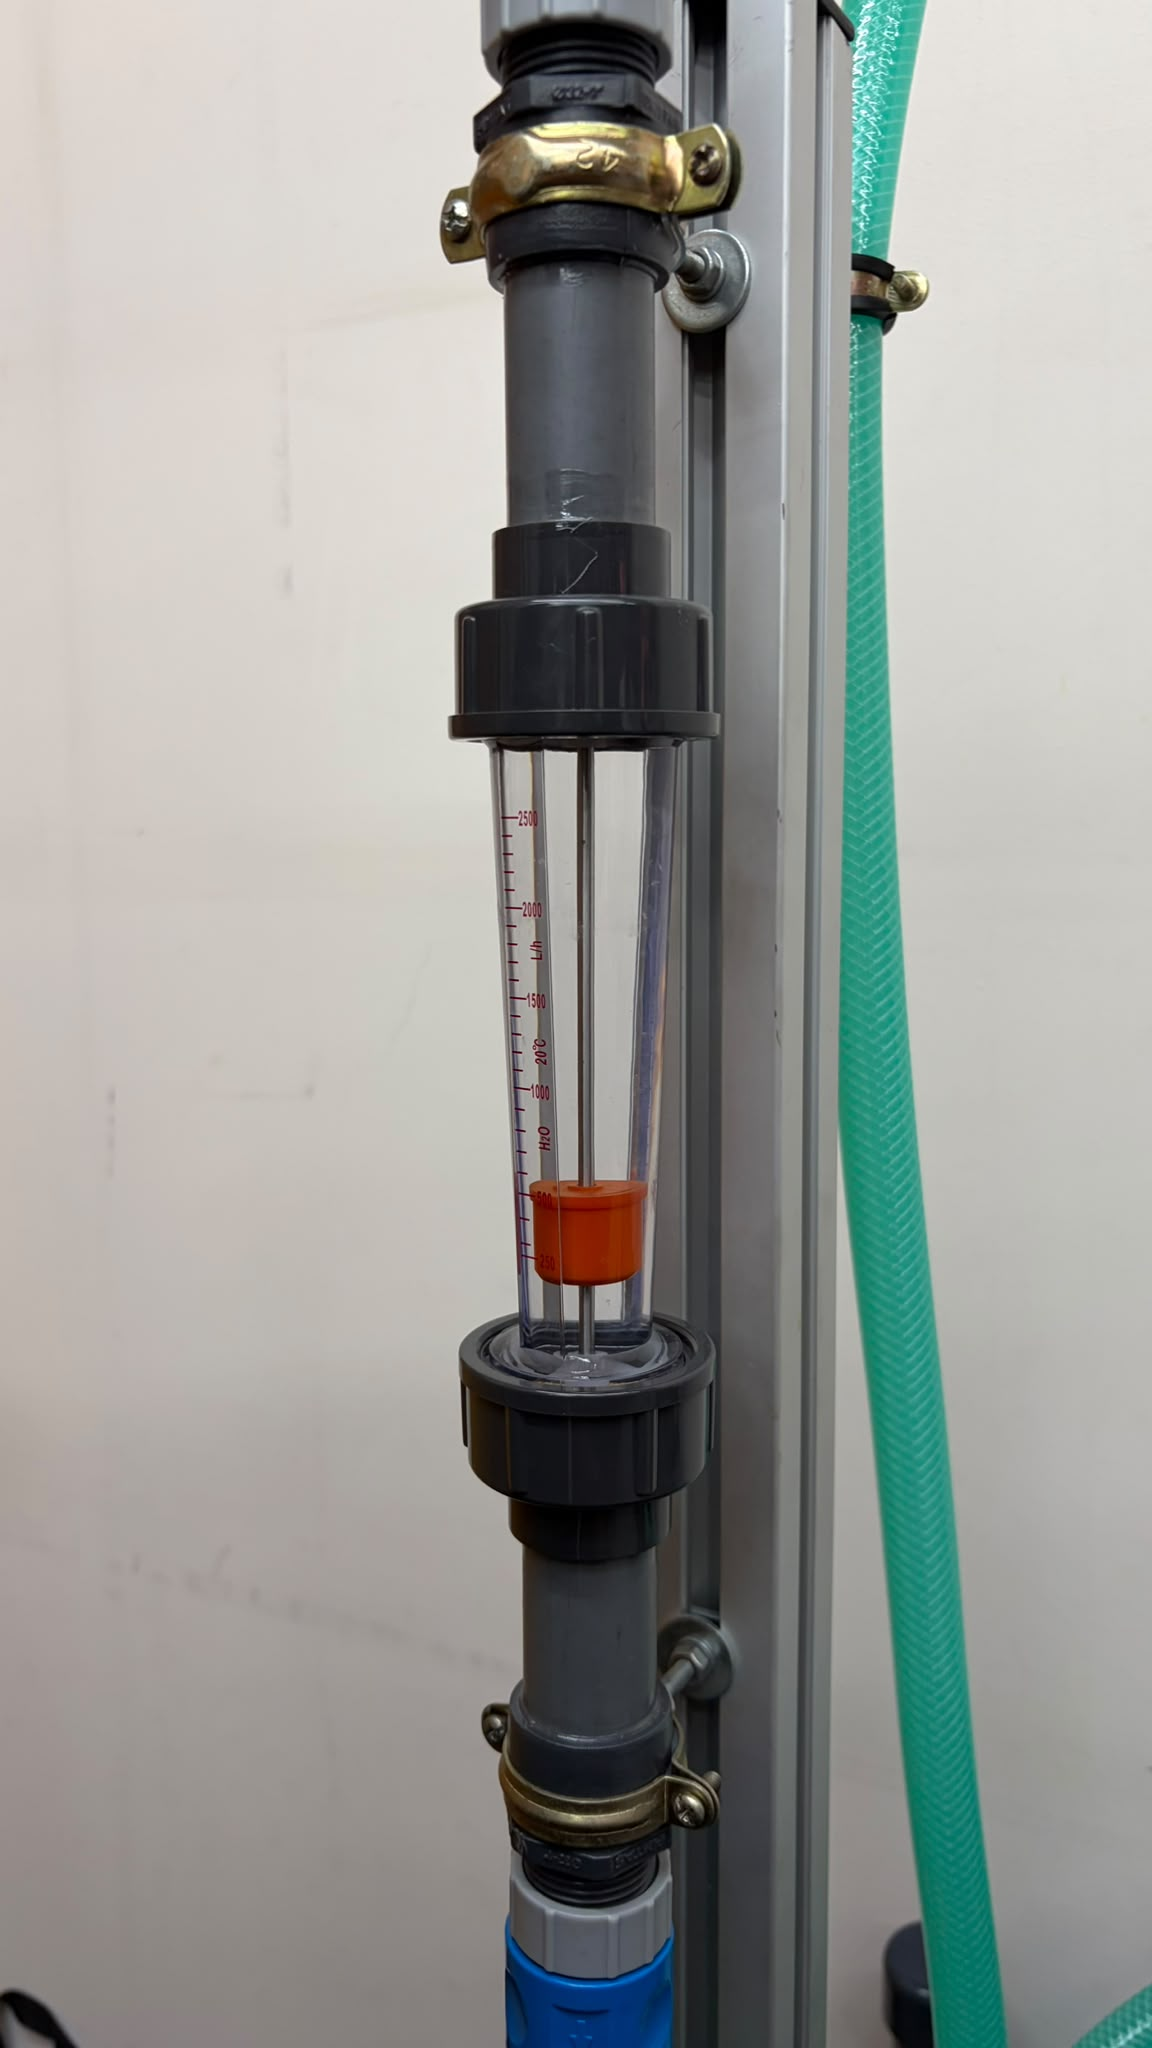
\includegraphics[height=4.5cm, width=\linewidth, keepaspectratio]{FlowMeter.jpeg}
        \caption{First flow condition}
        \label{fig:cd1}
    \end{subfigure}
    \hspace{0.05\textwidth}
    \begin{subfigure}[t]{0.35\textwidth}
        \centering
        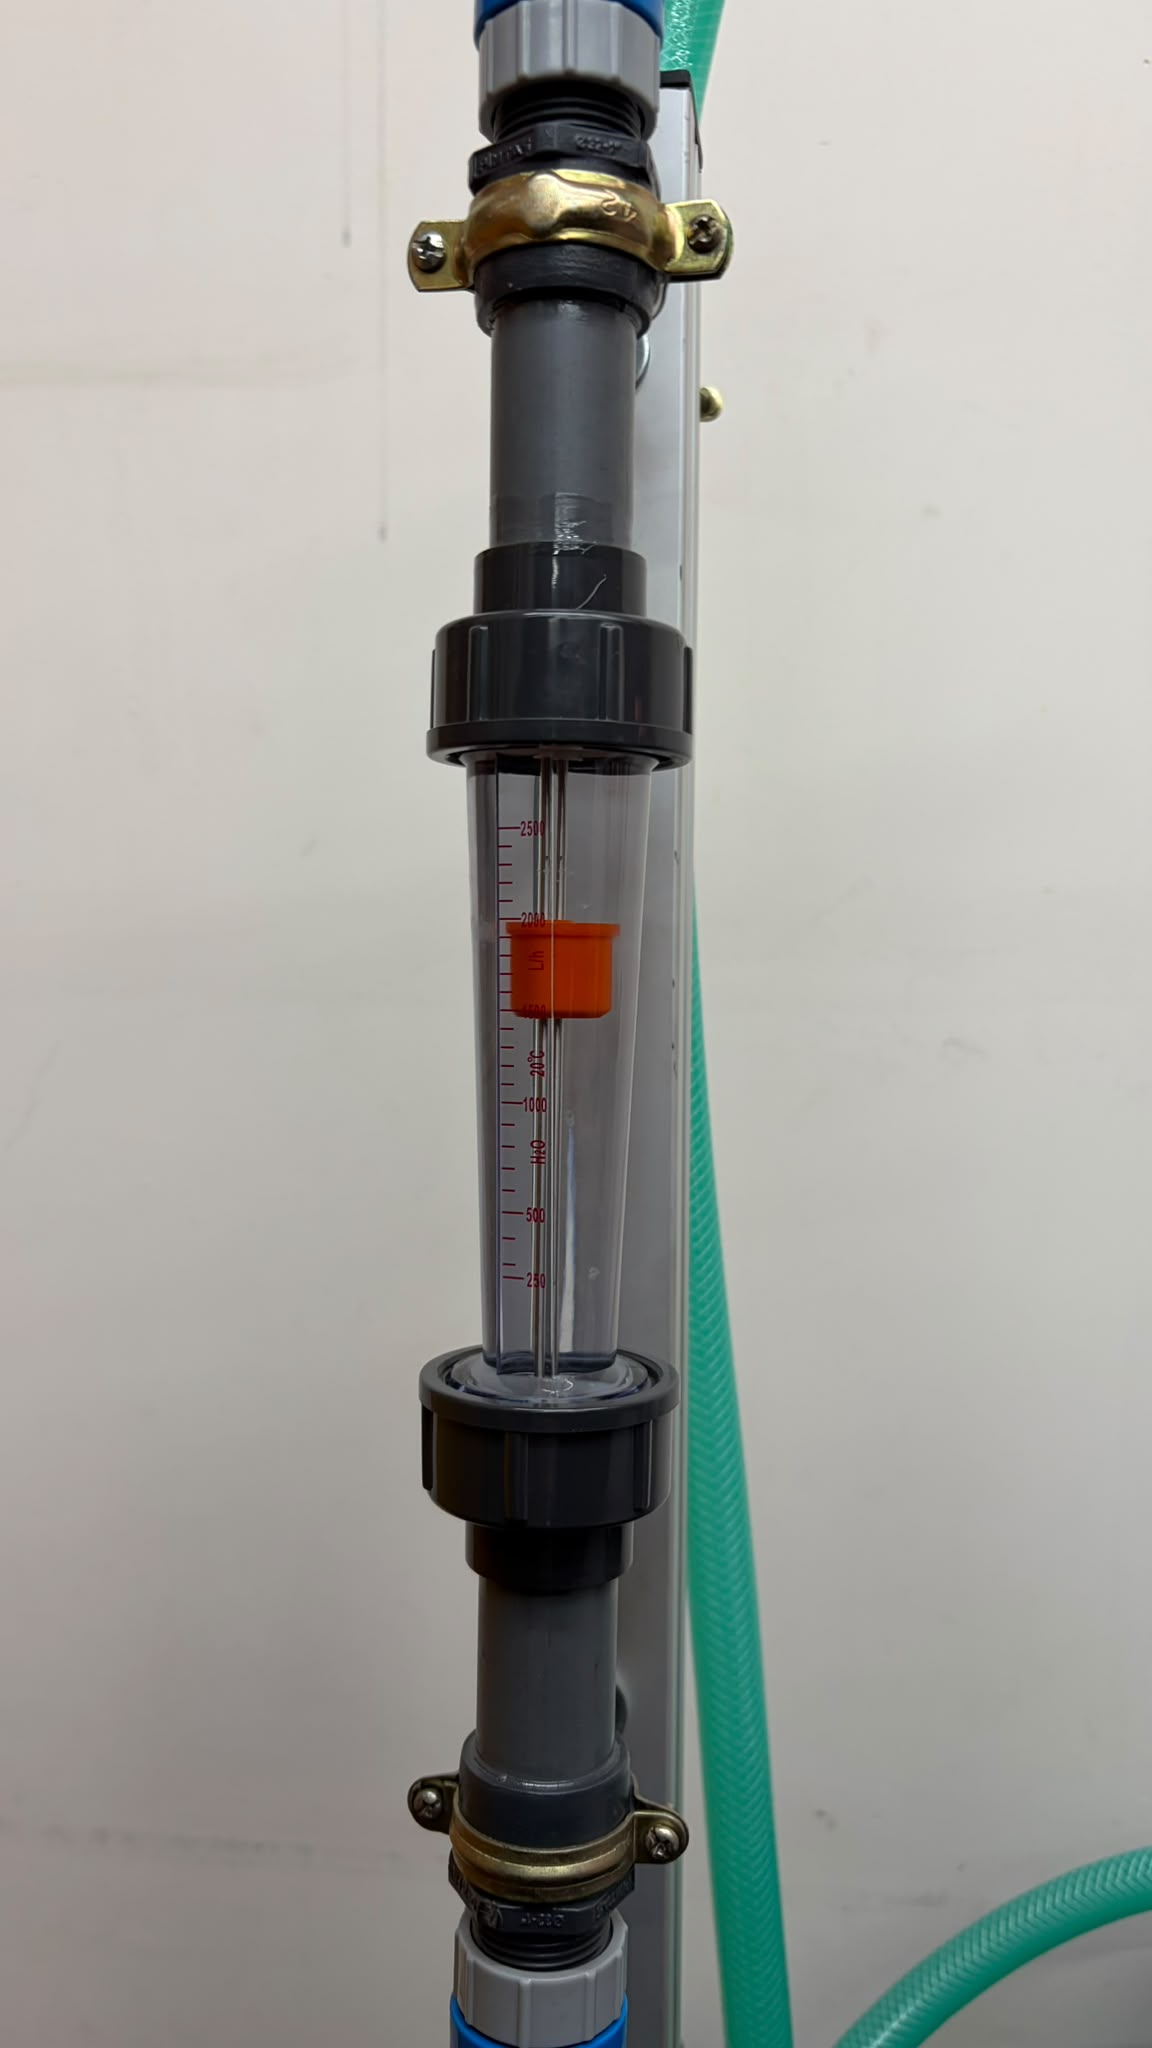
\includegraphics[height=4.5cm, width=\linewidth, keepaspectratio]{FlowMeter2.jpeg}
        \caption{Second flow condition}
        \label{fig:cd2}
    \end{subfigure}
    \caption{Flowmeter at different flow rates.}
    \label{fig:flowmeter_combined}
\end{figure}
  

\subsection{Procedure}

\begin{enumerate}[leftmargin=1.5em, itemsep=0.2em]
  \item Remove the cover of the transparent chamber, fix the flat plate to the vertical rod at the impact position and close the chamber.
  \item Place the module in the channel of the bench, connect its water inlet to the pump and level the assembly.
  \item Adjust the dial gauge until it is at the same height as the mark of the auxiliary platform.
  \item Select a fixed flow rate at which the dial gauge stops being at equilibrium (500 L/h in all three parts of our experiment)
  \item Place a calibrated mass on the platform, see if the dial gauge reaches again the equilibrium point, if so, note down both values, if not, keep increasing the external load on the disk until it does.
  \item Once a measure has been noted down, increase the flow rate again (we did steps of 100 L/h), see if it surpasses the equilibrium point and repeat the loading process from step 5.
  \item Repeat the whole procedure with the oblique deflector and the hemispherical cup.
\end{enumerate}\textbf{\textit{Note}}: the procedure followed in the lab is not the same as the one presented in the laboratory guidelines, which explains why our results are not the most accurate.

In the data set of this report, we obtained eleven equilibrium points for each obstacle, with flow rates from \SI{1500}{\litre\per\hour} to \SI{500}{\litre\per\hour} in steps of \SI{100}{\litre\per\hour}. The fluid properties used are $\rho=\SI{1000}{\kilogram\per\metre\cubed}$, $\mu=\SI{1.0e-3}{\pascal\second}$ and $g=\SI{9.81}{\metre\per\second\squared}$, giving $A=\SI{5.027e-5}{\metre\squared}$.

%% ================================================================ 4 DATA REDUCTION
\section{Data Reduction and Uncertainty Processing}

All data least-squares fits and figures were produced with MATLAB. The flow rate is converted to SI units, $Q_{\mathrm{SI}}=Q_{\mathrm{l/h}}/(3.6\times10^{6})$ (in \si{\metre\cubed\per\second}), and then $v=Q/A$, $\Red=\rho vd/\mu$, $F=W=(m/1000)\,g$ and $\Cd$ from Eq.~\eqref{eq:cd_definition}. Table~\ref{tab:kin} lists the kinematic and hydrodynamic variables. The Froude number based on the nozzle-to-surface distance ranges from $4.7$ to $14.1$, and $\Red$ from $2.2\times10^4$ to $6.6\times10^4$, so the hypotheses of high $\Red$ held throughout, while $\mathrm{Fr}\gg1$ is only satisfied at low flow rates.

\begin{table}[htbp]
\centering
\small
\caption{Kinematic and hydrodynamic variables of the jet ($d=\SI{8}{\milli\metre}$).}
\label{tab:kin}
\begin{tabular}{S[table-format=4.0] S[table-format=1.4] S[table-format=1.3] S[table-format=5.0] S[table-format=1.3]}
\toprule
{$Q$ (l/h)} & {$Q$ ($10^{-4}$ m$^3$/s)} & {$v$ (m/s)} & {$\Red$} & {$\rho Q^2/A$ (N)} \\
\midrule
1500 & 4.1667 & 8.289 & 66315 & 3.454 \\
1400 & 3.8889 & 7.737 & 61894 & 3.009 \\
1300 & 3.6111 & 7.184 & 57473 & 2.594 \\
1200 & 3.3333 & 6.631 & 53052 & 2.210 \\
1100 & 3.0556 & 6.079 & 48631 & 1.857 \\
1000 & 2.7778 & 5.526 & 44210 & 1.535 \\
900 & 2.5000 & 4.974 & 39789 & 1.243 \\
800 & 2.2222 & 4.421 & 35368 & 0.982 \\
700 & 1.9444 & 3.868 & 30947 & 0.752 \\
600 & 1.6667 & 3.316 & 26526 & 0.553 \\
500 & 1.3889 & 2.763 & 22105 & 0.384 \\
\bottomrule
\end{tabular}
\end{table}

Tables~\ref{tab:flat}--\ref{tab:hemi} contain the reduced data of each obstacle: the calibrated mass $m$, the measured force $W$, the theoretical force $\Fth=\tfrac12\Cd^{\mathrm{th}}\rho Q^2/A$, the experimental drag coefficient with its uncertainty $\delta\Cd$ and the relative error $\varepsilon=(W-\Fth)/\Fth$.

\begin{table}[htbp]
\centering
\small
\caption{Flat plate (theory: $\Cd=2$). $\delta\Cd$ computed with $\delta m=\SI{25}{\gram}$ and $\delta Q=\SI{25}{\litre\per\hour}$.}
\label{tab:flat}
\begin{tabular}{c r r r r r r r}
\toprule
\# & {$Q$ (l/h)} & {$m$ (g)} & {$W$ (N)} & {$\Fth$ (N)} & {$\Cd$} & {$\delta\Cd$}\\
\midrule
1 & 1500 & 350 & 3.433 & 3.454 & 1.99 & 0.21\\
2 & 1400 & 300 & 2.943 & 3.009 & 1.96 & 0.23\\
3 & 1300 & 250 & 2.453 & 2.594 & 1.89 & 0.26\\
4 & 1200 & 250 & 2.453 & 2.210 & 2.22 & 0.31 \\
5 & 1100 & 200 & 1.962 & 1.857 & 2.11 & 0.36 \\
6 & 1000 & 200 & 1.962 & 1.535 & 2.56 & 0.45\\
7 & 900 & 150 & 1.472 & 1.243 & 2.37 & 0.53 \\
8 & 800 & 100 & 0.981 & 0.982 & 2.00 & 0.62\\
9 & 700 & 100 & 0.981 & 0.752 & 2.61 & 0.84 \\
10 & 600 & 50 & 0.491 & 0.553 & 1.78 & 1.04\\
11 & 500 & 0 & 0.000 & 0.384 & -- & --  \\
\bottomrule
\end{tabular}
\end{table}

\begin{table}[htbp]
\centering
\small
\caption{$30^\circ$ oblique deflector (theory: $\Cd=3$).}
\label{tab:oblique}
\begin{tabular}{c r r r r r r r}
\toprule
\# & {$Q$ (l/h)} & {$m$ (g)} & {$W$ (N)} & {$\Fth$ (N)} & {$\Cd$} & {$\delta\Cd$\\
\midrule
1 & 1500 & 400 & 3.924 & 5.181 & 2.27 & 0.2\\
2 & 1400 & 350 & 3.433 & 4.513 & 2.28 & 0.2\\
3 & 1300 & 350 & 3.433 & 3.891 & 2.65 & 0.2 \\
4 & 1200 & 300 & 2.943 & 3.316 & 2.66 & 0.3 \\
5 & 1100 & 250 & 2.453 & 2.786 & 2.64 & 0.3 \\
6 & 1000 & 200 & 1.962 & 2.303 & 2.56 & 0.4 \\
7 & 900 & 150 & 1.472 & 1.865 & 2.37 & 0.53 \\
8 & 800 & 150 & 1.472 & 1.474 & 3.00 & 0.69\\
9 & 700 & 100 & 0.981 & 1.128 & 2.61 & 0.8 \\
10 & 600 & 100 & 0.981 & 0.829 & 3.55 & 1.1 \\
11 & 500 & 50 & 0.491 & 0.576 & 2.56 & 1.5 \\
\bottomrule
\end{tabular}
\end{table}

\begin{table}[htbp]
\centering
\small
\caption{Hemispherical cup (theory: $\Cd=4$).}
\label{tab:hemi}
\begin{tabular}{c r r r r r r r}
\toprule
\# & {$Q$ (l/h)} & {$m$ (g)} & {$W$ (N)} & {$\Fth$ (N)} & {$\Cd$} & {$\delta\Cd$} \\
\midrule
1 & 1500 & 550 & 5.396 & 6.908 & 3.12 & 0.\\
2 & 1400 & 500 & 4.905 & 6.017 & 3.26 & 0. \\
3 & 1300 & 450 & 4.415 & 5.189 & 3.40 & 0. \\
4 & 1200 & 350 & 3.433 & 4.421 & 3.11 & 0. \\
5 & 1100 & 300 & 2.943 & 3.715 & 3.17 & 0. \\
6 & 1000 & 250 & 2.453 & 3.070 & 3.20 & 0. \\
7 & 900 & 200 & 1.962 & 2.487 & 3.16 & 0.5 \\
8 & 800 & 150 & 1.472 & 1.965 & 3.00 & 0.6 \\
9 & 700 & 100 & 0.981 & 1.504 & 2.61 & 0.8 \\
10 & 600 & 100 & 0.981 & 1.105 & 3.55 & 1. \\
11 & 500 & 50 & 0.491 & 0.768 & 2.56 & 1.5 \\
\bottomrule
\end{tabular}
\end{table}

\subsection{Uncertainty propagation}

The force is $F=mg$, so $\delta F=g\,\delta m$. The mass is read as the number of \SI{50}{\gram} weights that balances the jet, which means that the true force lies within 25 g of the recorded value; we therefore take $\delta m=\SI{25}{\gram}$ ($\delta F=\SI{0.245}{\newton}$) as the nominal value, and $\delta m=\SI{50}{\gram}$ ($\delta F=\SI{0.491}{\newton}$) as a conservative bound. The flow meter reading is assumed to be known within $\delta Q=\SI{25}{\litre\per\hour}$.

Taking logarithms of Eq.~\eqref{eq:cd_definition}, $\ln\Cd=\ln 2+\ln F+\ln A-\ln\rho-2\ln Q$, and differentiating,
\begin{equation}
  \frac{d\Cd}{\Cd}=\frac{dF}{F}-2\,\frac{dQ}{Q}.
\end{equation}
The worst-case (linear) propagation, which is the one used in the previous reports of this course, gives
\begin{equation}
  \delta\Cd=\Cd\left(\frac{\delta F}{F}+2\,\frac{\delta Q}{Q}\right)=\Cd\left(\frac{\delta m}{m}+2\,\frac{\delta Q}{Q}\right),
  \qquad
  \frac{\delta\Red}{\Red}=\frac{\delta Q}{Q}.
  \label{eq:dcd}
\end{equation}
For the flat plate at $Q=\SI{1500}{\litre\per\hour}$, $\delta m/m=25/350=7.1\%$ and $2\delta Q/Q=3.3\%$, so $\delta\Cd/\Cd=10.5\%$, i.e.\ $\Cd=1.99\pm0.21$. At $Q=\SI{600}{\litre\per\hour}$ ($m=\SI{50}{\gram}$) the mass term alone is $50\%$ and $\delta\Cd=1.04$ for $\Cd=1.78$. With $\delta m=\SI{50}{\gram}$ the corresponding values at \SI{1500}{\litre\per\hour} would be $\pm0.35$. Because $\delta F$ is constant while $F\propto Q^2$, the relative uncertainty grows rapidly as the flow rate decreases, and the points at low flow rate have little statistical weight. The uncertainties $\delta\Cd$ in Tables~\ref{tab:flat}--\ref{tab:hemi} use the nominal $\delta m$.

\subsection{Least-squares fits}

Since $F=c\,Q^2$ with $c=\tfrac12\Cd\,\rho/A$, the effective drag coefficient of each obstacle is obtained from a least-squares fit through the origin of $F$ against $Q^2$,
\begin{equation}
  c=\frac{\sum_k Q_k^2F_k}{\sum_k Q_k^4},\qquad \Cd^{\mathrm{eff}}=\frac{2A}{\rho}\,c ,
  \label{eq:fit}
\end{equation}
with the standard error of the slope $s_c=\sqrt{\sum_k(F_k-cQ_k^2)^2/\big[(n-1)\sum_kQ_k^4\big]}$ and the coefficient of determination $R^2=1-\sum_k(F_k-cQ_k^2)^2/\sum_k(F_k-\bar F)^2$. These fits give more weight to the high-flow points, where the relative uncertainty is lowest, than an arithmetic mean of the individual $\Cd$ values. Table~\ref{tab:fit} summarises the results; the quoted $\pm$ is the statistical error of the slope and does not include systematic effects.

\begin{table}[htbp]
\centering
\small
\caption{Least-squares slopes of $F=cQ^2$ (units of $c$: $10^{7}\,\si{\newton\second\squared\per\metre\tothe{6}}$) and effective drag coefficients.}
\label{tab:fit}
\begin{tabular}{l c c c c c}
\toprule
Surface & $c_{\mathrm{th}}$ & $c_{\exp}$ & $c_{\exp}/c_{\mathrm{th}}$ & $\Cd^{\mathrm{eff}}$ & $R^2$ \\
\midrule
Flat plate ($\Cd=2$) & 1.989 & 2.038 & 1.024 & $2.05\pm0.07$ & 0.955 \\
$30^\circ$ deflector ($\Cd=3$) & 2.984 & 2.448 & 0.820 & $2.46\pm0.07$ & 0.964 \\
Hemisphere ($\Cd=4$) & 3.979 & 3.180 & 0.799 & $3.20\pm0.04$ & 0.993 \\
\bottomrule
\end{tabular}
\end{table}

%% ================================================================ 5 RESULTS
\section{Results and Discussion}
 
Figure~\ref{fig:force}(a--c) shows the measured force against the flow rate together with the theoretical curves for the three obstacles, and Fig.~\ref{fig:force}(d--f) gives $\Cd$ as a function of $\Red$. Figure~\ref{fig:fq7} compares the experimental and theoretical data of $F$ as a function of $Q$ for the three tested surfaces. All figures were generated with MATLAB from the data of Tables~\ref{tab:flat}--\ref{tab:hemi}.
 
% ---------- FIGURE 2: seis subfiguras ----------
\begin{figure}[H]
  \centering
  % --- Fila 1: F vs Q ---
  \begin{subfigure}[t]{0.32\textwidth}
    \centering
    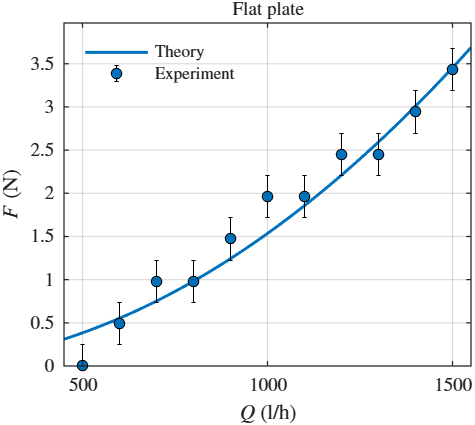
\includegraphics[width=\linewidth]{Figure_1.png}
    \caption{}
    \label{fig:fq1}
  \end{subfigure}\hfill
  \begin{subfigure}[t]{0.32\textwidth}
    \centering
    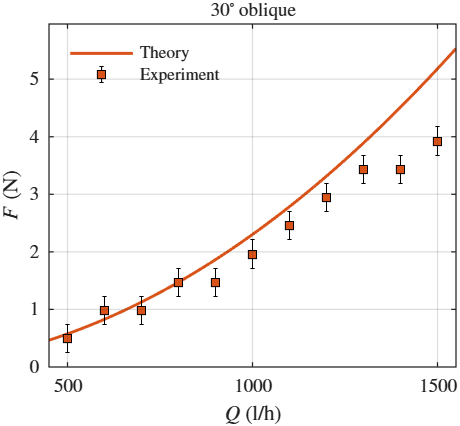
\includegraphics[width=\linewidth]{Figure_3.png}
    \caption{}
    \label{fig:fq2}
  \end{subfigure}\hfill
  \begin{subfigure}[t]{0.32\textwidth}
    \centering
    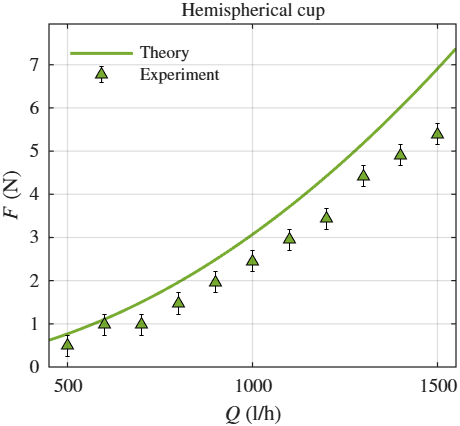
\includegraphics[width=\linewidth]{Figure_5.png}
    \caption{}
    \label{fig:fq3}
  \end{subfigure}
 
  \vspace{0.3em}
 
  % --- Fila 2: drag coefficient vs Reynolds ---
  \begin{subfigure}[t]{0.32\textwidth}
    \centering
    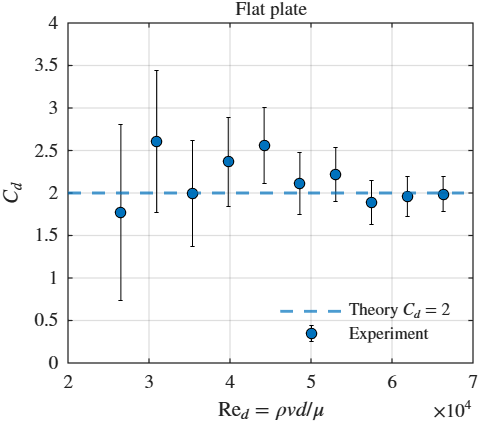
\includegraphics[width=\linewidth]{6.png}
    \caption{}
    \label{fig:cd1}
  \end{subfigure}\hfill
  \begin{subfigure}[t]{0.32\textwidth}
    \centering
    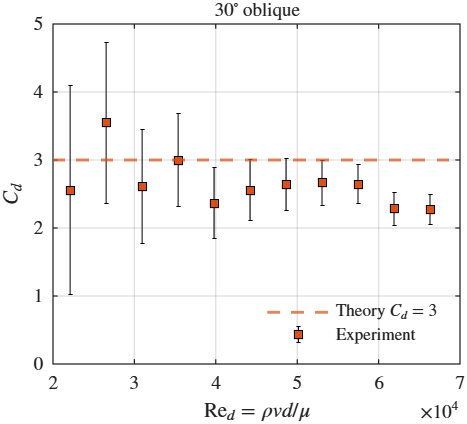
\includegraphics[width=\linewidth]{7.png}
    \caption{}
    \label{fig:cd2}
  \end{subfigure}\hfill
  \begin{subfigure}[t]{0.32\textwidth}
    \centering
    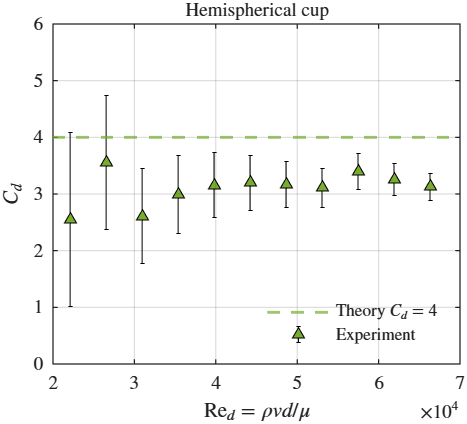
\includegraphics[width=\linewidth]{8.png}
    \caption{}
    \label{fig:cd3}
  \end{subfigure}
 
  \caption{Jet force on the three obstacles: flat plate, $30^\circ$ oblique plate and hemispherical cup (left to right). (a--c)~Force $F$ versus flow rate $Q$. (d--f)~Drag coefficient $C_D$ versus Reynolds number $\mathrm{Re}$. Markers: experiment (error bars in (a) and (d): $\pm\delta F$ with $\delta m=\SI{25}{\gram}$). Solid lines: theory, Eq.~\eqref{eq:general}. Horizontal error bars are present but not visible.}
  \label{fig:force}
\end{figure}
 
% ---------- FIGURE 3: imagen sola, centrada debajo ----------
\begin{figure}[H]
  \centering
  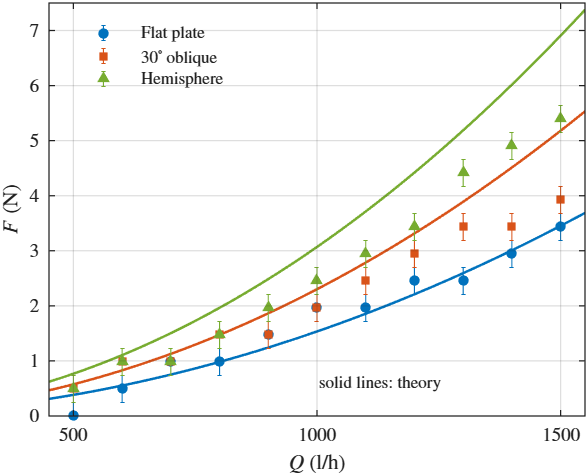
\includegraphics[width=0.40\textwidth]{Figure_7.png}
  \caption{Comparison of the experimental and theoretical data of $F$ as a function of $Q$ for the three tested surfaces.}
  \label{fig:fq7}
\end{figure}
 
% ---------- A PARTIR DE AQUÍ, SOLO TEXTO ----------
 
\textbf{Flat plate.} The experimental slope is $c_{\exp}=2.038\times10^{7}$ against the theoretical $1.989\times10^{7}$ (ratio $1.024$), i.e.\ $\Cd^{\mathrm{eff}}=2.05\pm0.07$ versus $2$. At the two highest flow rates the force is within $-0.6\%$ and $-2.2\%$ of the prediction, and nine of the ten non-zero points are compatible with $\Cd=2$ within $\delta\Cd$. At lower flow rates the individual errors reach $\pm30\%$, but they alternate in sign and are of the size expected from the \SI{50}{\gram} mass resolution (a single weight is $\SI{0.49}{\newton}$, comparable with $\Fth$ at $Q\le\SI{700}{\litre\per\hour}$). The flat plate therefore confirms Eq.~\eqref{eq:flat_force} within the experimental uncertainty.
 
\textbf{Oblique deflector.} The measured slope is $82\%$ of the theoretical one, $\Cd^{\mathrm{eff}}=2.46\pm0.07$ against $3$. The deficit is clear at high flow rate, where the measured force is $24\%$ below the prediction at $1500$ and \SI{1400}{\litre\per\hour} and $11$--$15\%$ below between $1300$ and \SI{1000}{\litre\per\hour}. Six of the eleven points are compatible with $\Cd=3$ within $\delta\Cd$; most of them lie at $Q\le\SI{900}{\litre\per\hour}$, where $\delta\Cd$ exceeds $0.5$ and the test is therefore weak.
 
\textbf{Hemispherical cup.} The slope is $80\%$ of the theoretical one, $\Cd^{\mathrm{eff}}=3.20\pm0.04$ against $4$. This is the best-defined fit ($R^2=0.993$) and the deficit, $-15\%$ to $-25\%$ over most of the range, is far larger than the experimental uncertainty. Only two points (those at 600 and \SI{500}{\litre\per\hour}, with $\delta\Cd>1$) are compatible with $\Cd=4$.
 
The unconstrained fits $F=aQ^2+b$ give intercepts $b=+0.04$, $+0.25$ and $-0.09\,\si{\newton}$ for the flat, oblique and hemispherical surfaces, all smaller than one \SI{50}{\gram} weight ($\SI{0.49}{\newton}$), so $F\propto Q^2$ is consistent with the data and the deficits are not due to a constant offset.
 
\subsection{Hierarchy of forces}
 
The theory predicts $F_{\text{flat}}:F_{30^\circ}:F_{\text{hemi}}=1:1.5:2$. In the data, $F_{\text{flat}}<F_{30^\circ}<F_{\text{hemi}}$ holds strictly at the five highest flow rates ($1500$ to \SI{1100}{\litre\per\hour}); at lower flow rates several readings coincide because of the \SI{50}{\gram} resolution (e.g.\ flat plate and oblique deflector both read $\SI{200}{\gram}$ at $\SI{1000}{\litre\per\hour}$, and all three read $\SI{100}{\gram}$ at $\SI{700}{\litre\per\hour}$), but the ordering $F_{\text{flat}}\le F_{30^\circ}\le F_{\text{hemi}}$ is never violated. The fitted slopes also follow this order strictly ($2.05<2.46<3.20$), although their ratios, $1:1.20:1.56$, are smaller than the ideal $1:1.5:2$.
 
\subsection{Reynolds-number dependence}
 
In Fig.~\ref{fig:force}(d--f) the flat-plate points scatter around $\Cd=2$ without a systematic trend with $\Red$. For the deflecting surfaces $\Cd$ is below the ideal value throughout, with larger scatter at low $\Red$ (low force) caused by the mass quantisation. Over the narrow range of $\Red$ covered ($2.2$--$6.6\times10^{4}$) the data do not show a clear Reynolds dependence beyond the scatter.

%% ================================================================ 6 ERRORS
\section{Physical Sources of Error and Discrepancy Diagnostics}

The forces measured on the oblique deflector and in the hemisphere are below the ideal ones, which means $\Cd<\Cd^{\mathrm{th}}$. The following points are the reasons why these discrepancies appear:

\begin{enumerate}[leftmargin=1.5em, itemsep=0.4em]
  \item \textbf{Gravitational deceleration of the jet.} The jet travels vertically $h\approx\SI{35}{\milli\metre}$ before it reaches the obstacle, so the impact velocity is $v_{\mathrm{imp}}=\sqrt{v_0^2-2gh}$. So, the reduction of force is $F/F_0\approx 1-2gh/v_0^2$, which is $1.0\%$ at $\SI{1500}{\litre\per\hour}$ and $9\%$ at $\SI{500}{\litre\per\hour}$ ($\mathrm{Fr}=14.1$ and $4.7$). This effect explains only a small part of the $20\%$ deficit at high flow rate (it would also affect the flat plate, which agrees with theory), and it increases the deviation mainly at low flow rate.
  \item \textbf{Interference of the return curtain.} In the hemisphere, the sheet is turned downward and falls around the jet inside the test cylinder. The falling sheet can hit the incoming jet and mix with it, or splash back onto the cup. Because of this, the water does not change its direction completely, and the exit velocity is not fully downward. The oblique deflector has a similar effect, but to a smaller extent. As a result, the change in vertical momentum is reduced.
  \item \textbf{Quantisation of the weights.} The masses are added step by step adding \SI{50}{\gram} each time, what corresponds to $\delta W=\SI{0.4905}{\newton}$. Theoretically, at low flow rates the force itself should be of the order of one or two weights, so then, the relative resolution obtained at the laboratory is poor: the flat plate at \SI{500}{\litre\per\hour} ($\Fth=\SI{0.384}{\newton}$, less than one weight) registered \SI{0}{\gram}. This is consistent with the force not being able to overcome static friction of the lever mechanism or with a small residual tare of the balance; in either case the zero reading is a resolution limit and not evidence against the model. It also explains the large $\pm30\%$ scatter of individual errors at low flow.
  \item \textbf{Viscous boundary-layer effects.} In a real flow, the water sheet loses some speed because of friction with the walls of the obstacle. We can describe this with a velocity coefficient $c_v<1$, so that the water leaves the obstacle with speed $c_v v$ instead of $v$. The force then becomes $F=\rho Q v\,(1+c_v\sin\theta)$. If we match this expression to the measured $\Cd^{\mathrm{eff}}$, we need $c_v\approx0.46$ for the oblique deflector and $c_v\approx0.60$ for the cup. This means that the water would lose about $54\%$ and $40\%$ of its speed, which is too much to be caused by friction alone in a thin sheet at $\Red\sim10^{4}$--$10^5$. Friction therefore plays a role, together with items 1, 2 and 4 and with an exit angle smaller than the ideal one, but it cannot explain the whole difference by itself.
 \item \textbf{Deviation from the prescribed measurement procedure.} The laboratory guide prescribes fixing the mass on the platform and regulating the flow rate until equilibrium, so that the flow meter, which can be read continuously, supplies the measured quantity at each point and the weight $W=mg$ is known exactly. In the session the opposite was done: the flow rate was fixed at a round value and the masses were adjusted until the platform was balanced. In principle both procedures sample the same curve $F(Q)$, but they place the resolution differently.
\end{enumerate}

%% ================================================================ 7 CONCLUSIONS
\section{Conclusions}

\begin{itemize}[leftmargin=1.5em, itemsep=0.3em]
  \item Applying the Reynolds Transport Theorem to a control volume with Bernoulli's equation on the free surface and mass conservation gives $F=\rho Q^2(1+\sin\theta)/A$, i.e.\ $\Cd=2,\,3,\,4$ for the flat plate, the $30^\circ$ deflector and the hemisphere.
  \item The measured forces scale as $Q^2$ for the three obstacles ($R^2=0.955$, $0.964$, $0.993$), and the order of the forces, flat plate $\le$ oblique $\le$ hemisphere, is reproduced at all flow rates.
  \item For the flat plate the theory is confirmed: $\Cd^{\mathrm{eff}}=2.05\pm0.07$, with the force within $2.2\%$ of the prediction at \SI{1400}{\litre\per\hour} and above.
  \item For the $30^\circ$ deflector and the hemisphere the measured drag coefficients, $2.46\pm0.07$ and $3.20\pm0.04$, are about $18$--$20\%$ below the ideal values. The ideal model is therefore an upper bound for these geometries. The main candidates are interference of the return flow, viscous losses and incomplete turning of the sheet, with gravitational deceleration of the jet adding a few per cent at low flow rate.
  \item The mass resolution of \SI{50}{\gram} limits the accuracy at low flow rate, where the relative uncertainty of $\Cd$ exceeds $50\%$. A finer set of weights, or a longer measurement at high flow rates, would be the most effective improvement of the experiment.
\end{itemize}
In summary, the integral momentum balance captures the scaling and the hierarchy of the jet forces, and gives a quantitative prediction for the flat plate, while for strongly deflecting surfaces it should be complemented with loss coefficients to describe a real jet.

%% ================================================================ REFERENCES
\begin{thebibliography}{9}
\bibitem{white} F.~M. White, \textit{Fluid Mechanics}, 8th ed., McGraw-Hill Education, 2016.
\bibitem{notes} A.~L. S\'anchez and J.~Rodr\'iguez-Rodr\'iguez, \textit{Engineering Fluid Mechanics: Course Notes}, Universidad Carlos III de Madrid, Departamento de Ingenier\'ia T\'ermica y de Fluidos.
\bibitem{guide} Departamento de Ingenier\'ia T\'ermica y de Fluidos, \textit{Jet Impact on Surfaces: Laboratory Guide}, Engineering Fluid Mechanics, Universidad Carlos III de Madrid.
\end{thebibliography}

\section*{Tools used}
\begin{itemize}[leftmargin=1.5em, itemsep=0.2em]
  \item MATLAB: data reduction, least-squares fits and all figures (\texttt{process\_\allowbreak lab1\_\allowbreak data.m}).
  \item Overleaf: preparation of the document.
\end{itemize}

\end{document}
